\chapter{Testy Funkcjonalne}
\section{Integracja bloku filtra w projekcie}

W celu sprawdzenia integralności wykonanego bloku, zestawiono układ jak na Rysunku \ref{fig:itest}.
Test integracyjny ma wykazać czy występuje zgodność typów danych we/wyj oraz zgodność panelu konfiguracyjnego użytkownika.
Jeżeli nastąpi próba łączenia niekompatybilnych ze sobą bloków, wyświetli się błąd podobny do tego z~Rysunku \ref{fig:error}.
Po podłączeniu bloków, środowisko nie zgłasza alarmów co oznacza, że filtr może przyjmować dane ze źródła USRP. 
Panel parametrów wyświetla się prawidłowo i wymaga od użytkownika podania kluczowych parametrów.
  
\begin{figure}[ht]
\centering
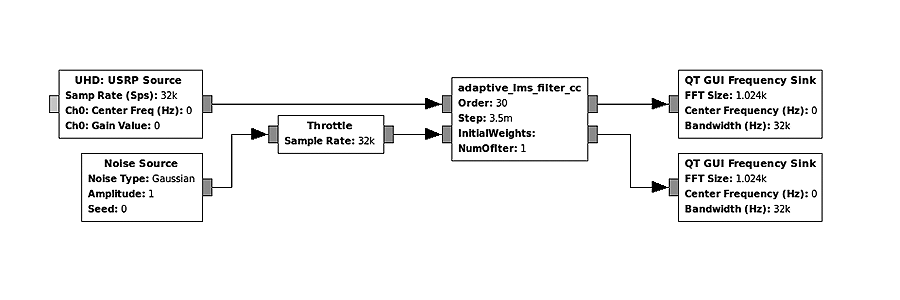
\includegraphics[scale=1.1]{ch5_integration.png}
\caption{Układ do testu integracyjnego}
\label{fig:itest}
\end{figure}

\section{Eliminacja zakłóceń sinusoidalnych}

\begin{figure}[ht]
\centering
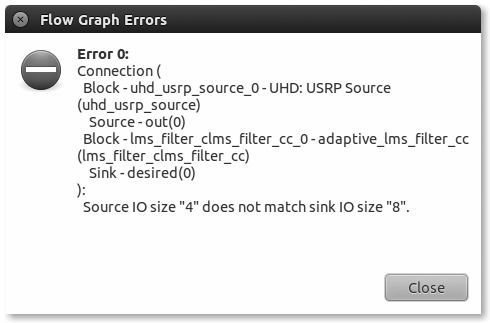
\includegraphics[scale=0.7]{ch5_error.png}
\caption{Błąd projektu informujący o niezgodności typów danych.}
\label{fig:error}
\end{figure}
\subsection{Weryfikacja poprawności działania}

\paragraph{Test 1.}
Wygenerowano 1kHz szum pasmowy, który imituje sygnał danych.
Sygnał został zsumowany z falą zakłócającą o częstotliwości $2kHz$.
Suma została podana na wejście główne filtra, a do wejścia odniesienia podłączono źródło sygnału sinusoidalnego o tej samej częstotliwości co składowa zakłócająca, lecz innej fazie.
Częstotliwość sinusoid zwiększano stopniowo.

\paragraph{Obserwacja 1.}
Na Wykresie \ref{fig:sine1} przedstawiono efekt filtracji sygnału.
Zakłócenie  zostało pomyślnie odfiltrowane.
Moc w paśmie użytecznym została wyrównana.

\begin{figure}[ht]
\centering
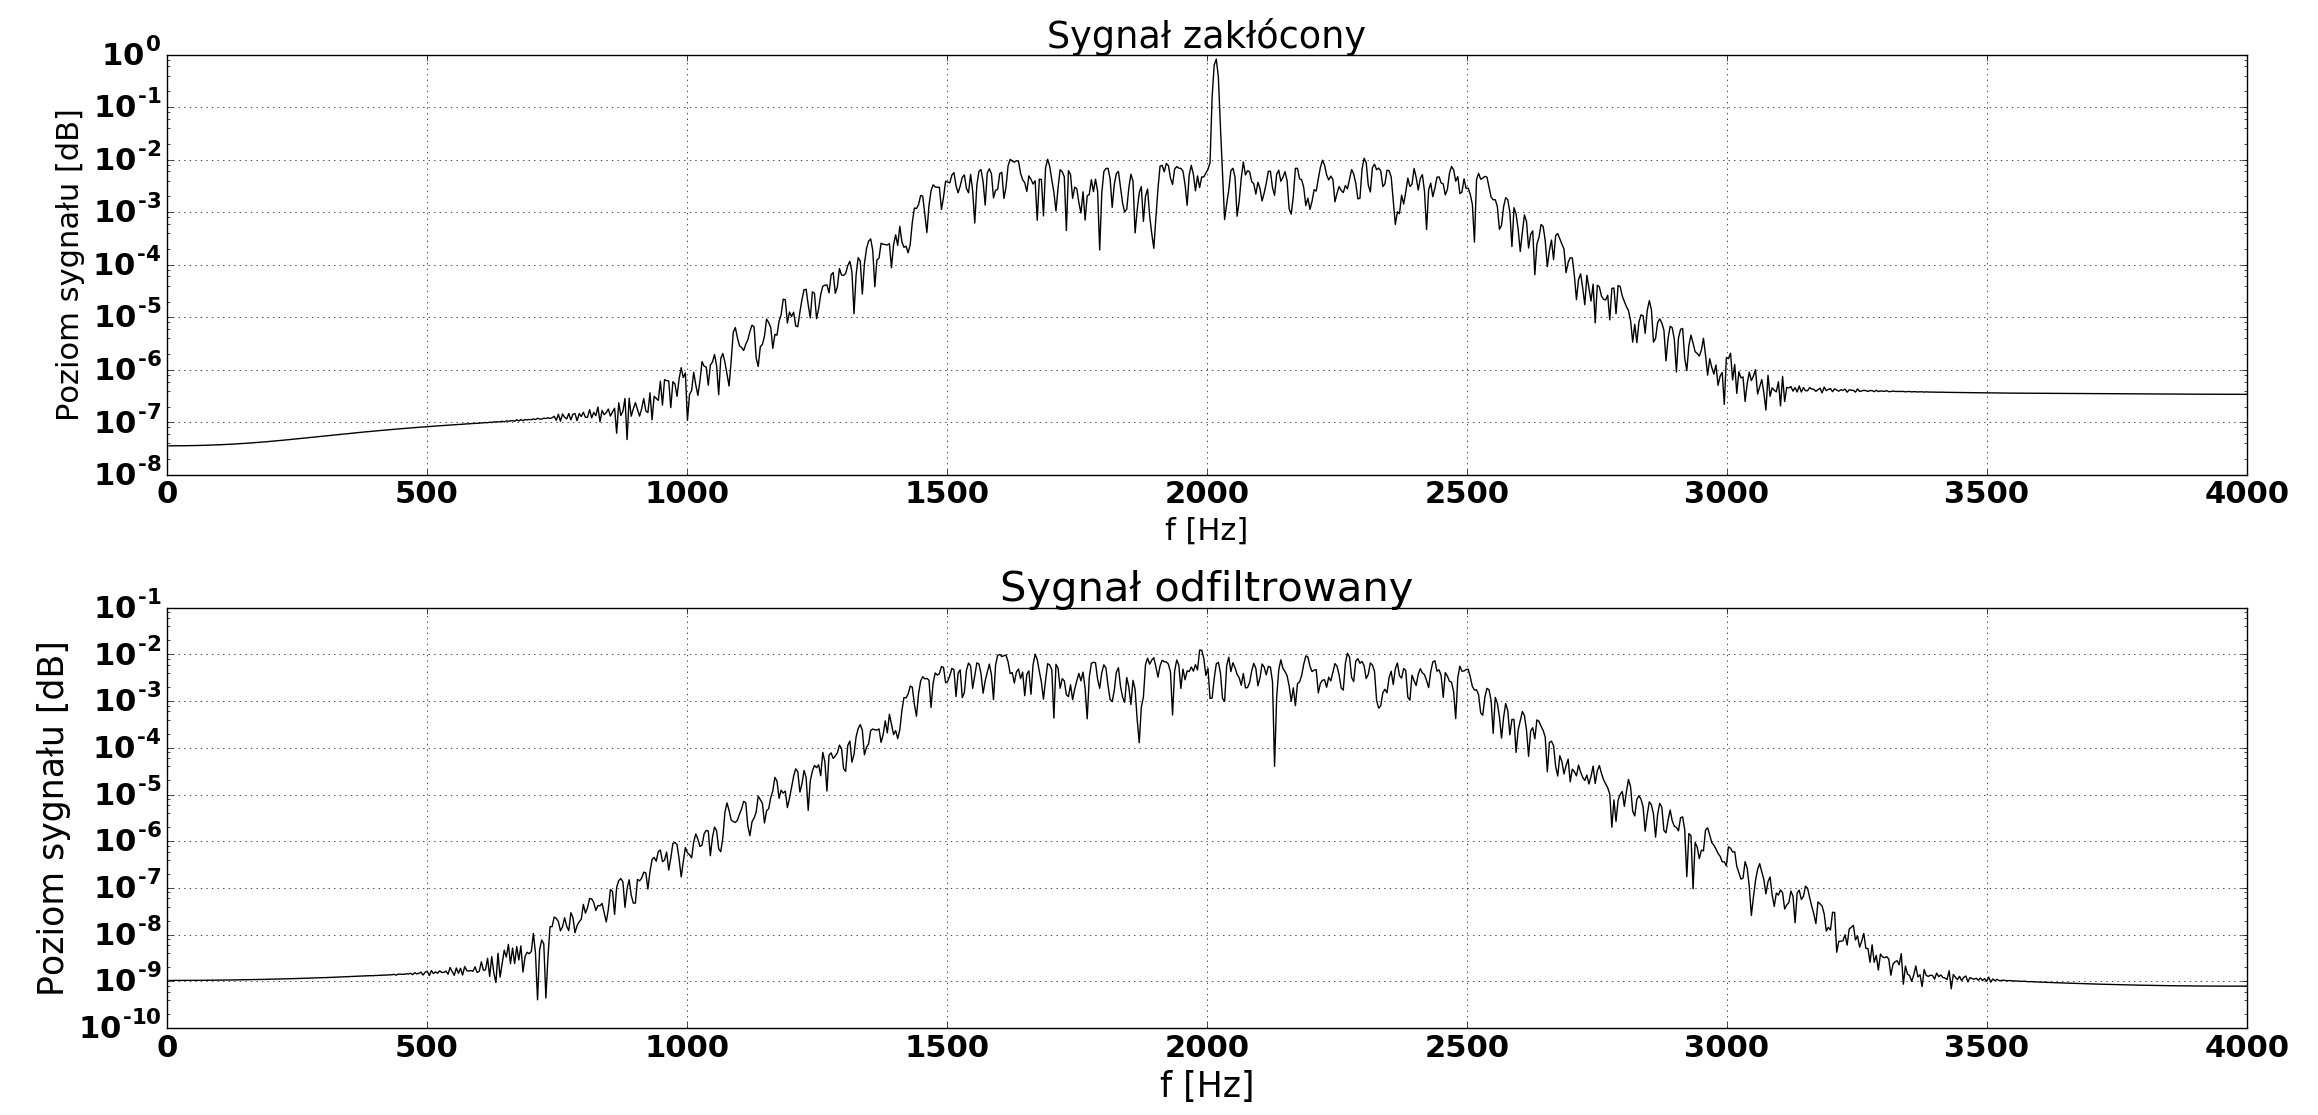
\includegraphics[scale=0.27]{sine1}
\caption{Filtracja zakłóceń o częstotliwości 2kHz}
\label{fig:sine1}
\end{figure}

\paragraph{Obserwacja 2.}
Kiedy częstotliwość zakłócenia osiągnęła wartość wykraczającą poza pasmo użyteczne sygnału, zakłócenie znacznie wyróżniało się na wykresie widma. (Rysunek \ref{fig:sine2})
Moc sinusoidy o częstotliwości 3kHz została stłumiona względem niefiltrowanego sygnału o ok. 20dB.
Świadczy to o tym, że algorytm podąża za zmianami sygnału interferującego.

\begin{figure}[ht]
\centering
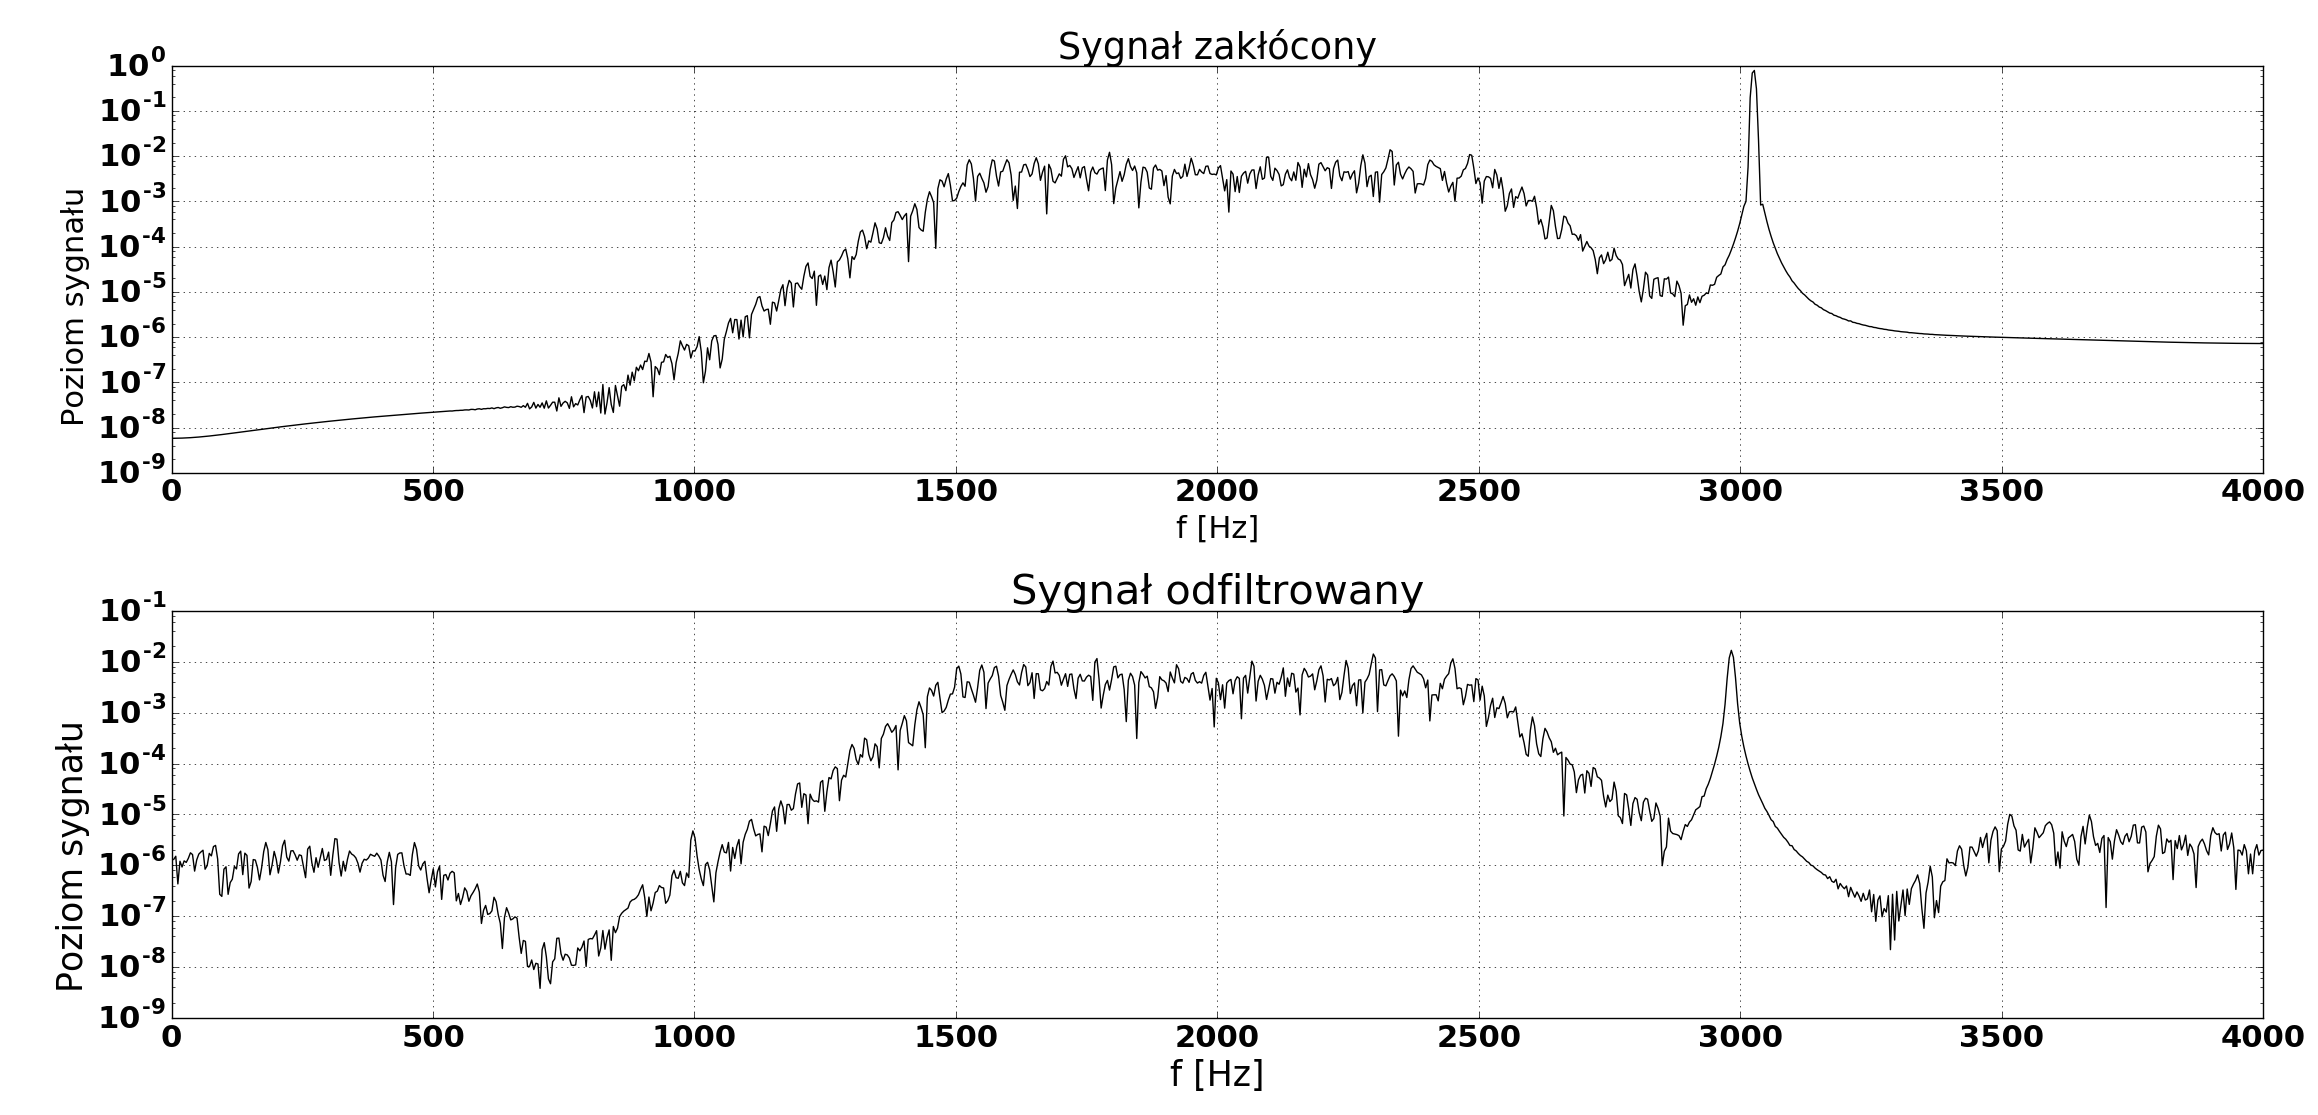
\includegraphics[scale=0.27]{sine2}
\caption{Filtracja zakłóceń o częstotliwości 3kHz}
\label{fig:sine2}
\end{figure}

\paragraph{Test 2.}
Podobnie jak w teście 1. wykorzystano szum pasmowy i sinusoidalny sygnał zakłócający.
Zmieniając wartość kroku adaptacji filtra zbadano jego wpływ na kształt widma.
Dla każdej z wartości kroku obliczono wartość bezwzględną błędu estymacji.

\paragraph{Obserwacja 3.}
Im większy jest parametr kroku $\mu$, tym szybsze są możliwości śledzenia przez filtr adaptacyjny (Rysunek \ref{fig:sine4}). Duży parametr kroku $\mu$ może sprowadzać niakceptowalnie duży błąd średniokwadratowy. \cite{Haykin:1998:ST} 
Przykładem tego są wyraźnie obserwowalne na rys. \ref{fig:sine3} zaniki w widmie, na częstotliwości odpowiadającej cz. sygnału zakłócającego.

\begin{figure}[ht]
\centering
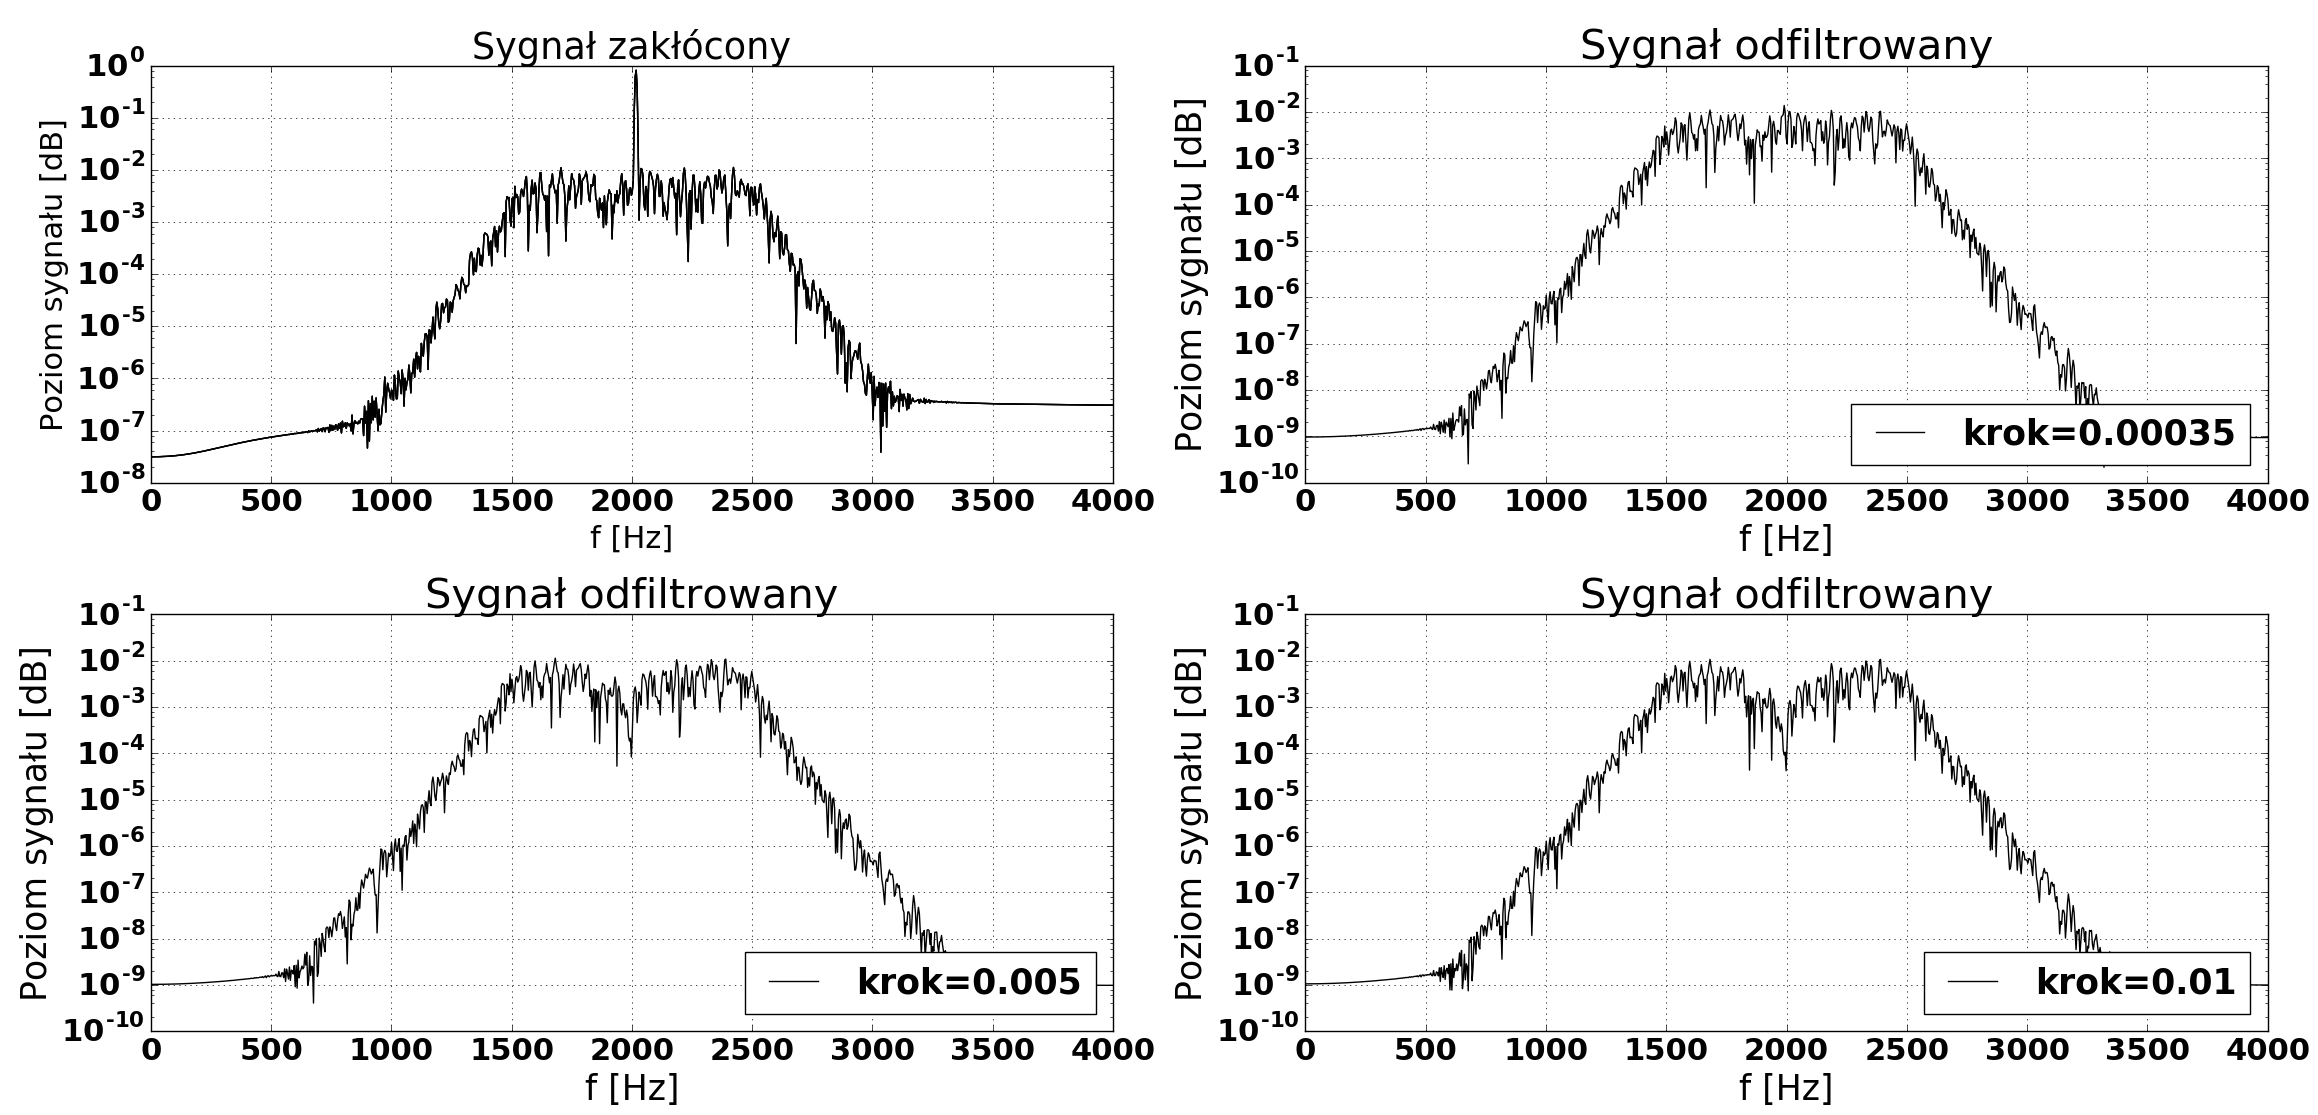
\includegraphics[scale=0.27]{sine3}
\caption{Wpływ parametru kroku na widmo sygnału.}
\label{fig:sine3}
\end{figure}

\begin{figure}[ht]
\centering
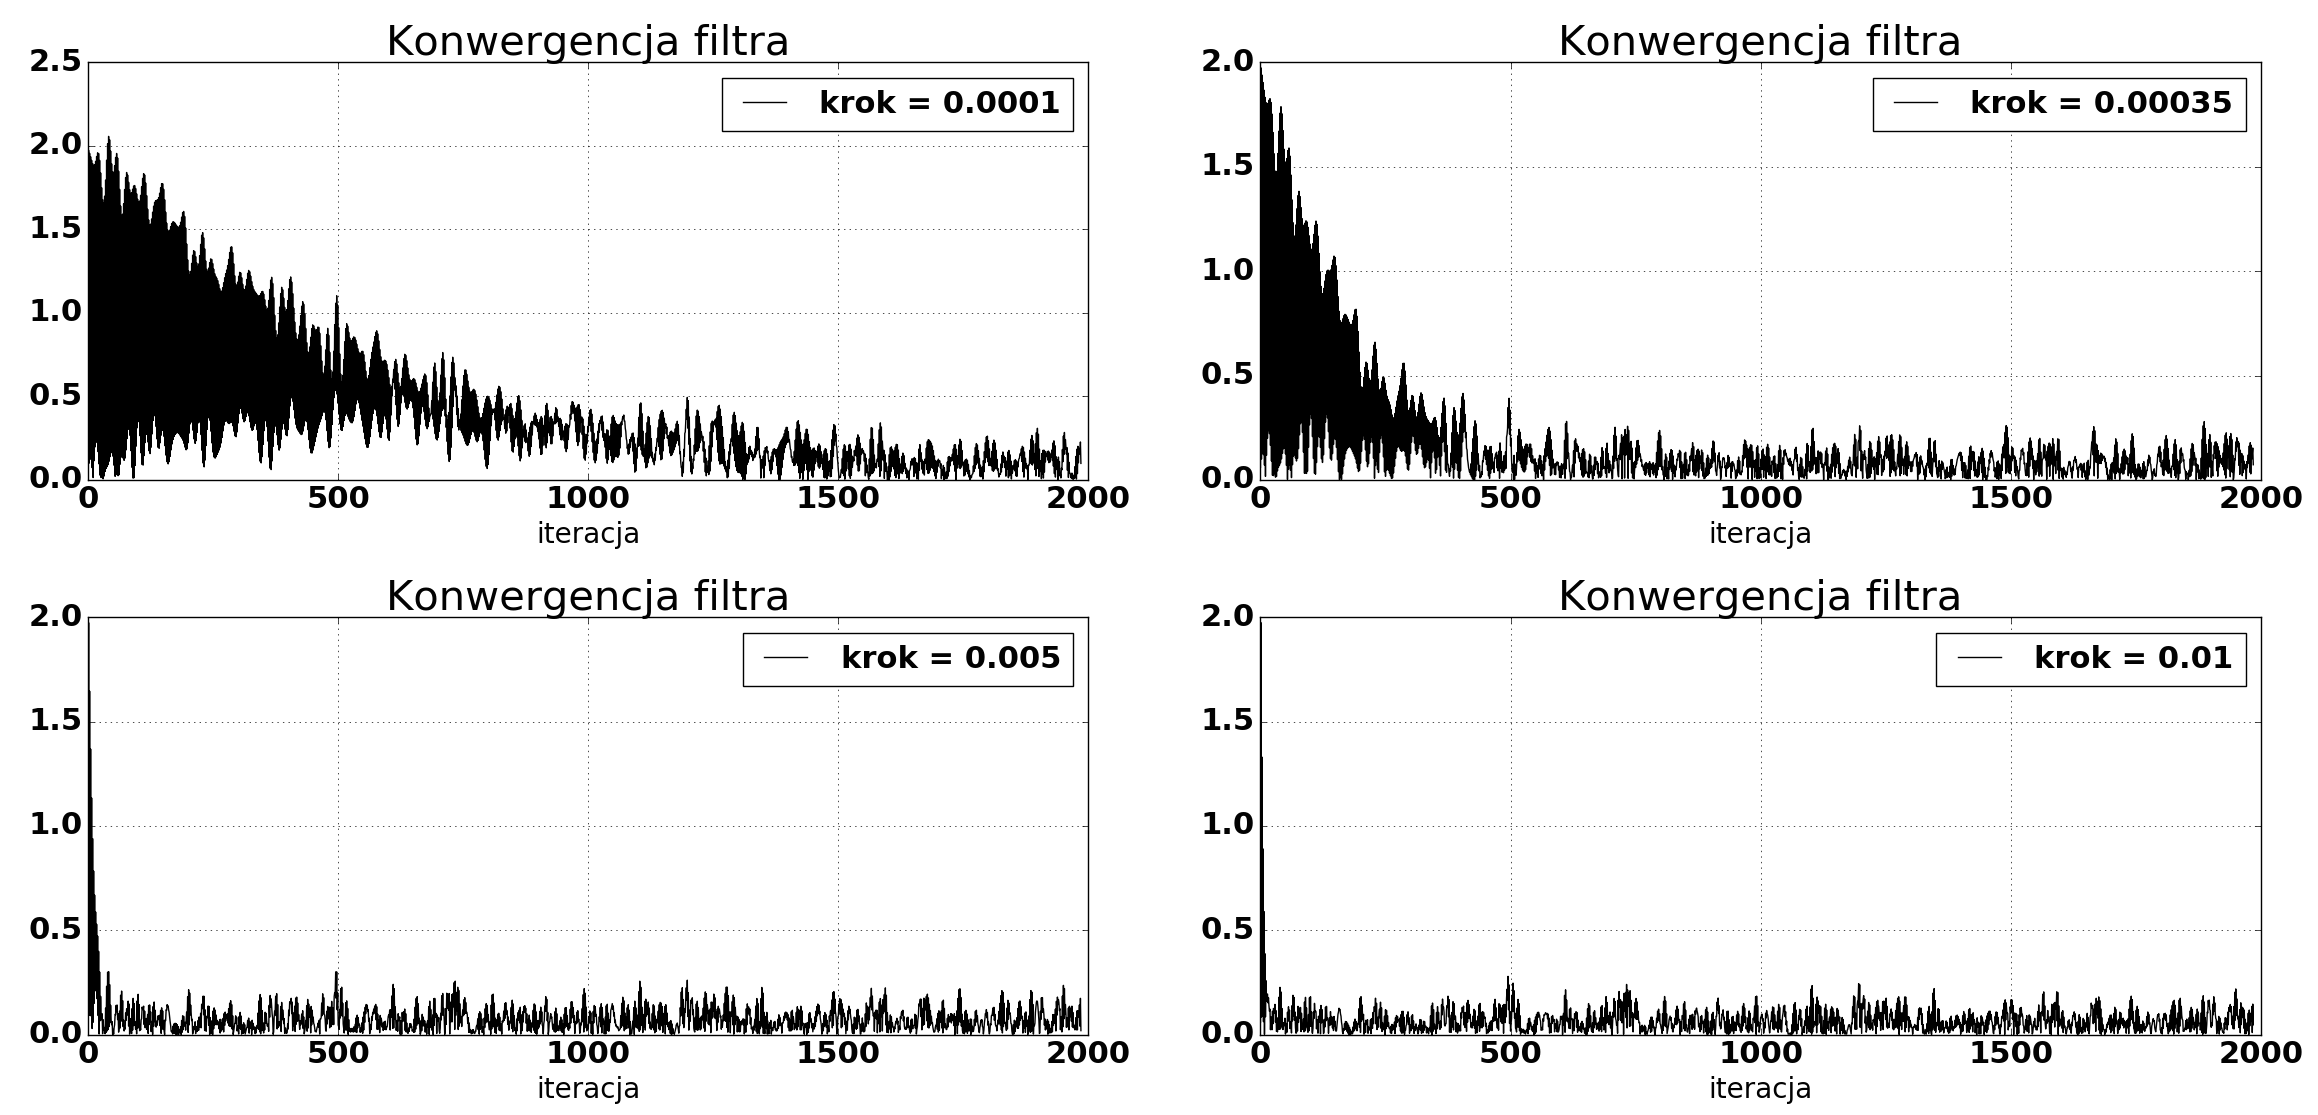
\includegraphics[scale=0.27]{konwergencja}
\caption{Wpływ parametru kroku na szybkość zbieżności algorytmu.}
\label{fig:sine4}
\end{figure}

\section{Korekcja adaptacyjna}

Przedstawione w Tabeli \ref{eqnoeq} schematy konfiguracji odbiornika zostały stworzone do testów.
Jedna z korektorem na bazie algorytmu LMS, druga bez korektora w celu porównania wydajności modułu \texttt{LMS DD Equalizer}. 
Skrót \texttt{DD} pochodzi od ang. \textit{Decision Directed} co oznacza, że punktem odniesienia dla algorytmu jest obiekt konstelacji zawierający mapę symboli sygnału. \cite{dd_lms_eq}

\begin{sidewaystable}[t]
\centering
\caption{Diagramy konfiguracji odbiornika}
\label{eqnoeq}
\begin{tabular}{l}
\hline
Transmisja bez korekcji \\
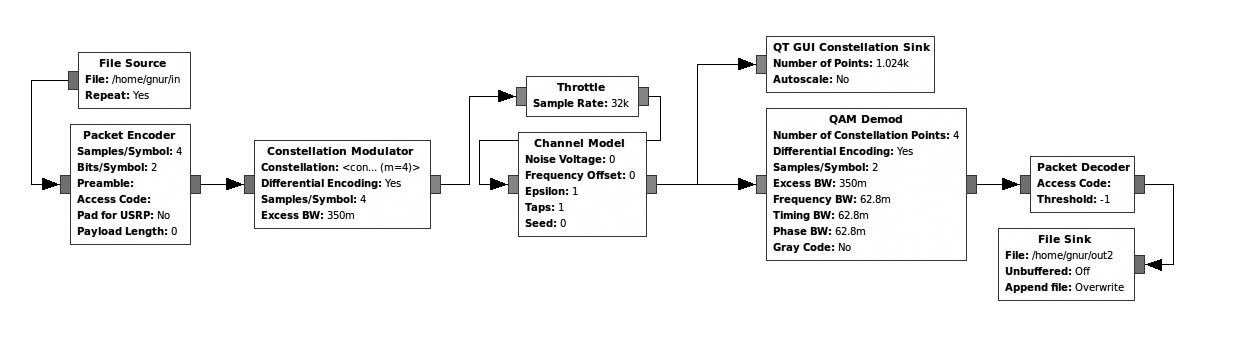
\includegraphics[scale=0.5]{noeq.png}\\ \hline
Transmisja z korekcją   \\
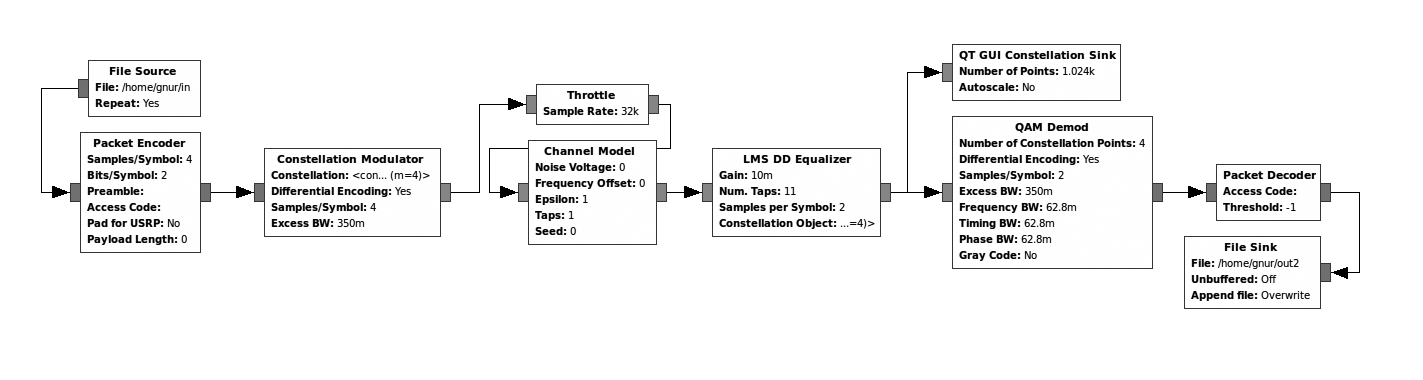
\includegraphics[scale=0.5]{eq.png}\\
\end{tabular}
\end{sidewaystable}

\paragraph{Test 1.}
Zbadana została skuteczność eliminacji zakłóceń w postaci addytywnego białego szumu.
Wartość amplitudy szumu jest jednym z parametrów bloku \texttt{Channel Model}.
Celem było przesłanie pliku graficznego ze źródła do ujścia z wykorzystaniem modulacji QPSK i modelu kanału radiowego.


\begin{table}[ht]
\centering
\caption{Konfiguracja bez korektora}
\label{tab:noeq}
\begin{tabular}{|l|l|l|}
\hline
0mV      & 150mV    & 200mV    \\
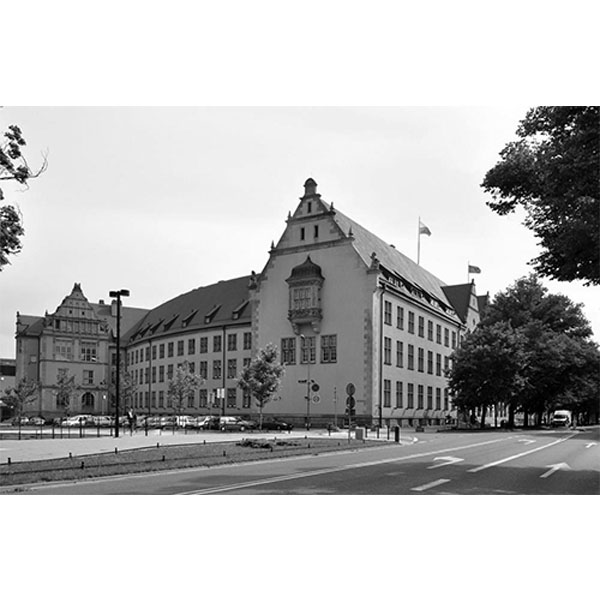
\includegraphics[scale=0.45]{a1origin} & 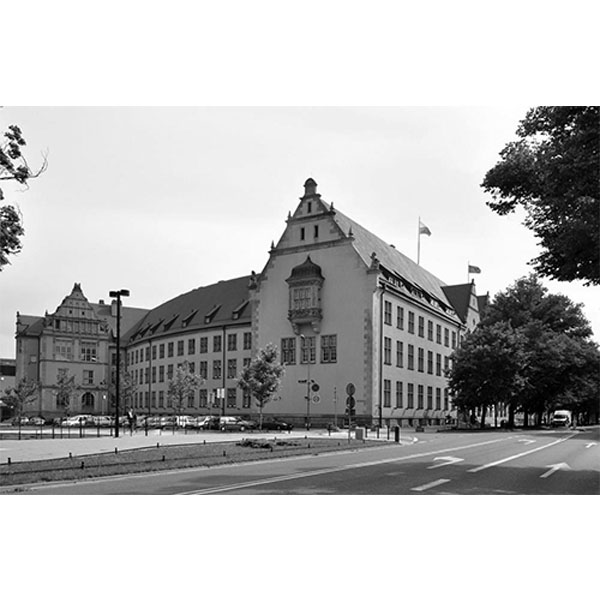
\includegraphics[scale=0.45]{a1origin} & 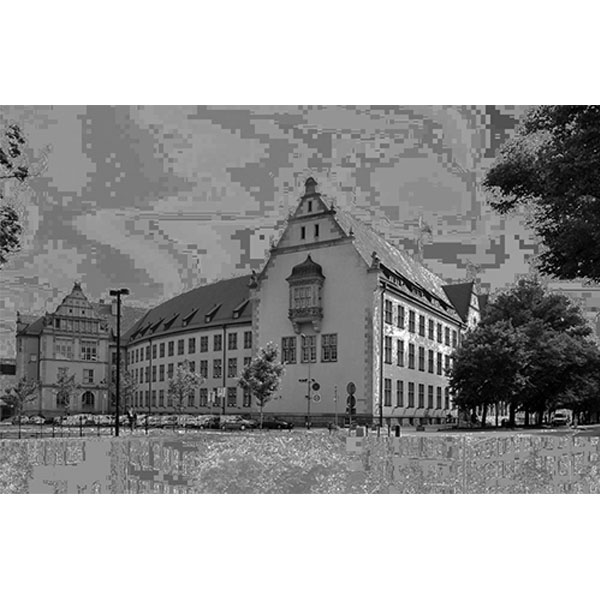
\includegraphics[scale=0.45]{noeq200mva1} \\
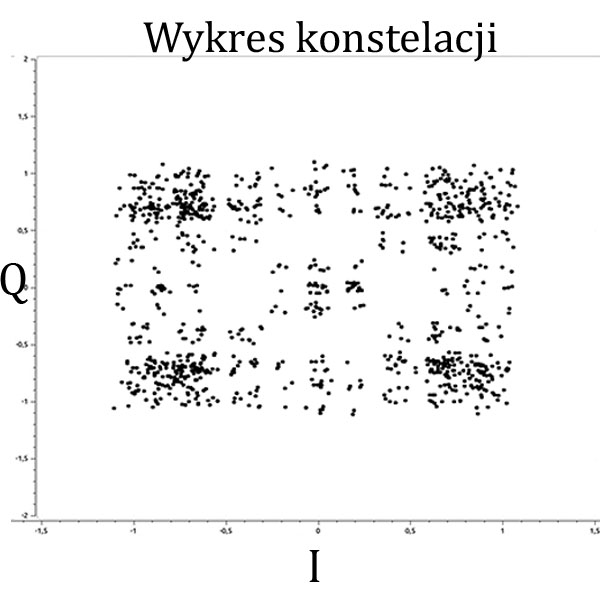
\includegraphics[scale=0.45]{noeq0mv}   & 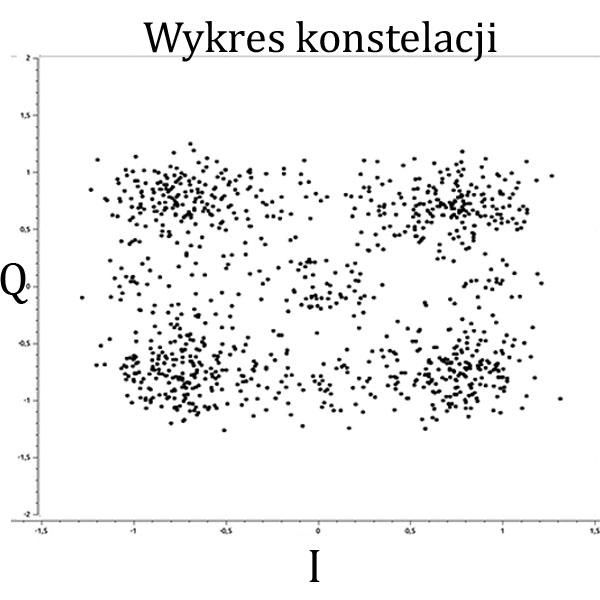
\includegraphics[scale=0.45]{noeq150mv}   & 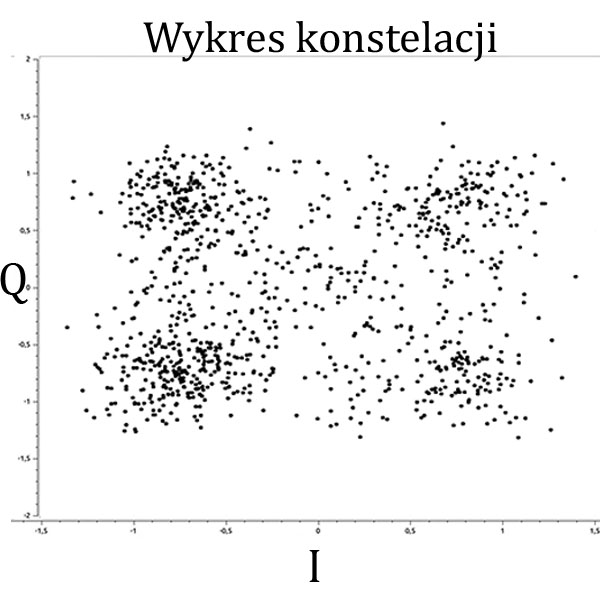
\includegraphics[scale=0.45]{noeq200mv}  \\ \hline
\end{tabular}
\end{table}

\paragraph{Obserwacja 1.}
Na podstawie wyników zawartych w Tabeli \ref{tab:noeq} stwierdzono, że im większy poziom szumu addytywnego w kanale, tym gorszy stosunek S/N. 
Skutkuje to rozmyciem się konstelacji i błędnym rozpoznawaniem symboli w dekoderze.
Efektem tego jest zniekształcony obraz na wyjściu. 


\begin{table}[ht]
\centering
\caption{Konfiguracja z korektorem}
\label{tab:eq}
\begin{tabular}{|l|l|l|}
\hline
0mV      & 200mV    & 250mV    \\
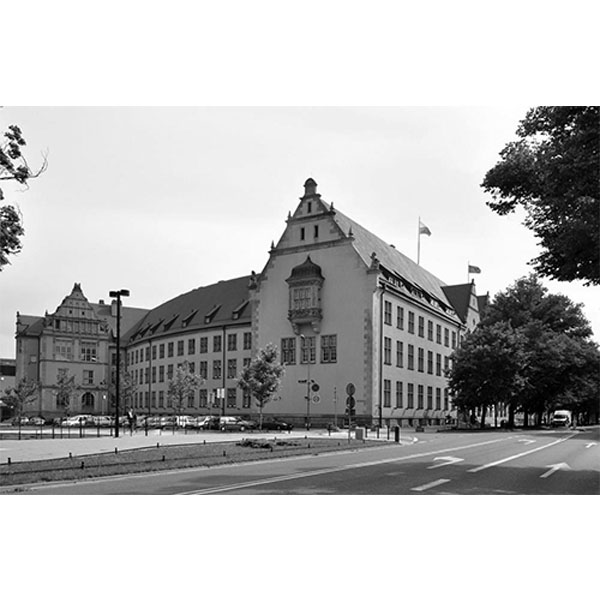
\includegraphics[scale=0.45]{a1origin} & 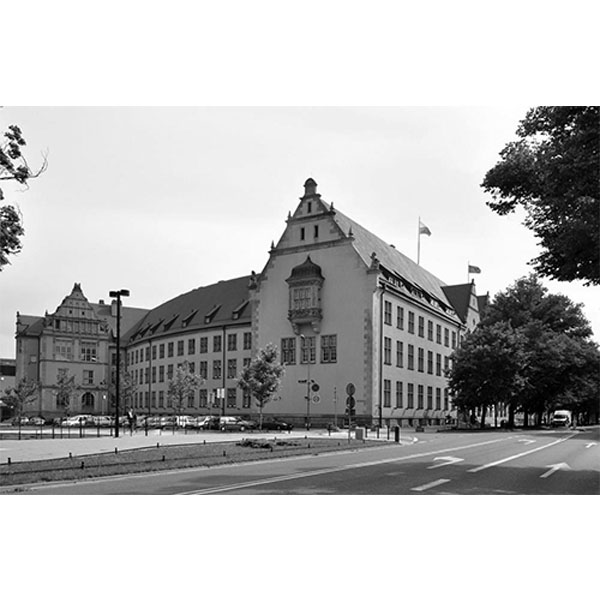
\includegraphics[scale=0.45]{a1origin} & 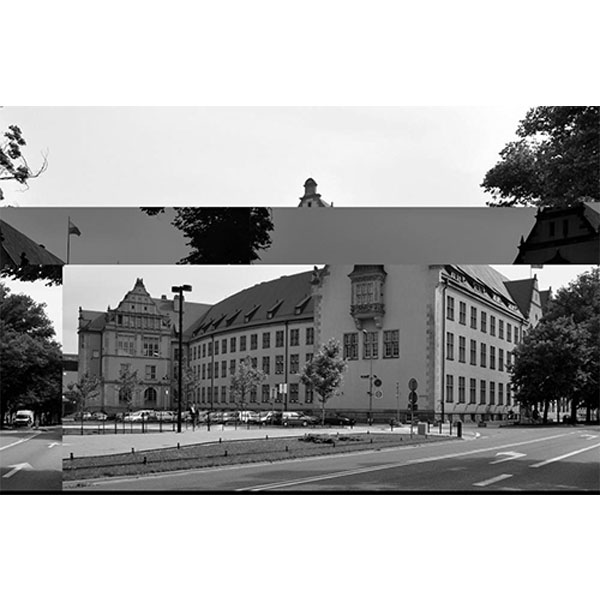
\includegraphics[scale=0.45]{eq250mva1} \\
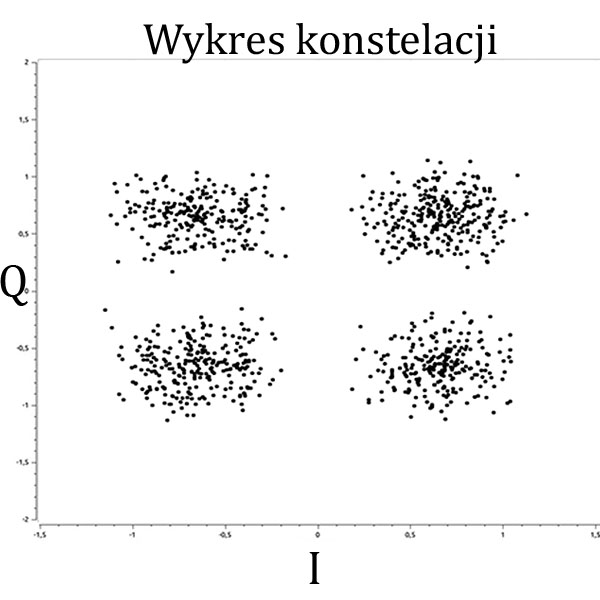
\includegraphics[scale=0.45]{eq0mv}   & 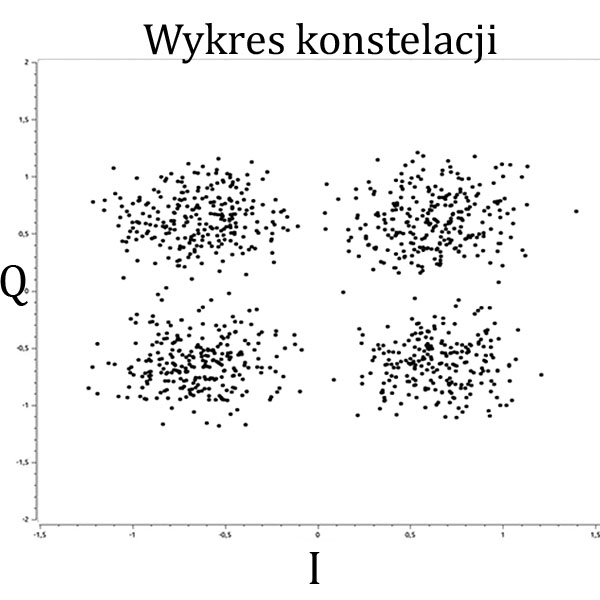
\includegraphics[scale=0.45]{eq200mv}   & 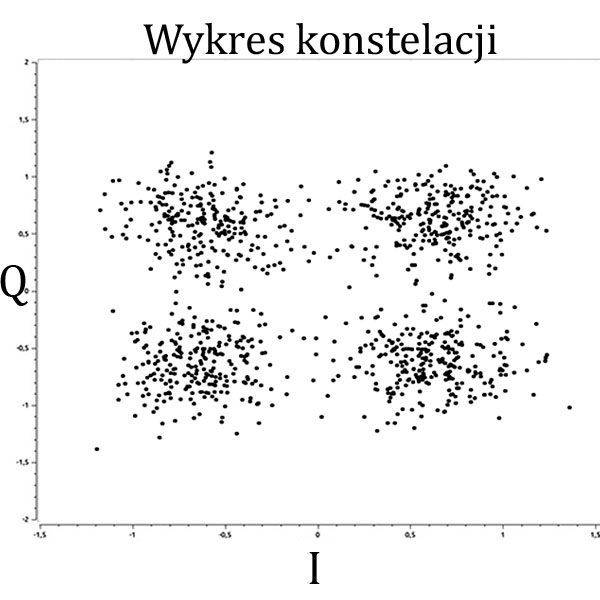
\includegraphics[scale=0.45]{eq250mv}  \\ \hline
\end{tabular}
\end{table}

\paragraph{Obserwacja 2.}
Tabela \ref{tab:eq} zawiera wyniki próby z korekcją szumu.
Korektor wpływa na wykres konstelacji, lepiej separując symbole przy tym samym poziomie szumu.
Dekoder z korektorem przestaje poprawnie interpretować dane przy poziomie szumu powyżej $250mV$.

\paragraph{Test 3.}
Zbadano jakość korekcji modelu kanału przez blok \texttt{LMS DD Equalizer}.
W~tabeli \ref{channel_eq} umieszczono wykresy charakterystyk kanału dla przypadku z korekcją i~bez.
Model kanału jest filtrem o pewnej odpowiedzi impulsowej.
Zadaniem korektora jest zniwelowanie efektów kanału oddziałujących na sygnał.
Wykres charakterystyki powstał poprzez wpuszczenie białego szumu na wejście kanału i obliczenie dyskretnej transformaty Fouriera z jego wyjścia.

\paragraph{Obserwacja 1.}
Wykres konstelacji informuje o wielkości zniekształceń sygnału, które dla kanału bez korekcji są znacznie większe niż dla kanału z korekcją.
Algorytm LMS efektywnie eliminuje zakłócenia związane z degradacją sygnału w kanale radiowym.


\begin{table}[ht]
\centering
\caption{Korekcja kanału}
\label{channel_eq}
\begin{tabular}{|c|c|}
\hline
Kanał bez korekcji & Kanał z korekcją \\
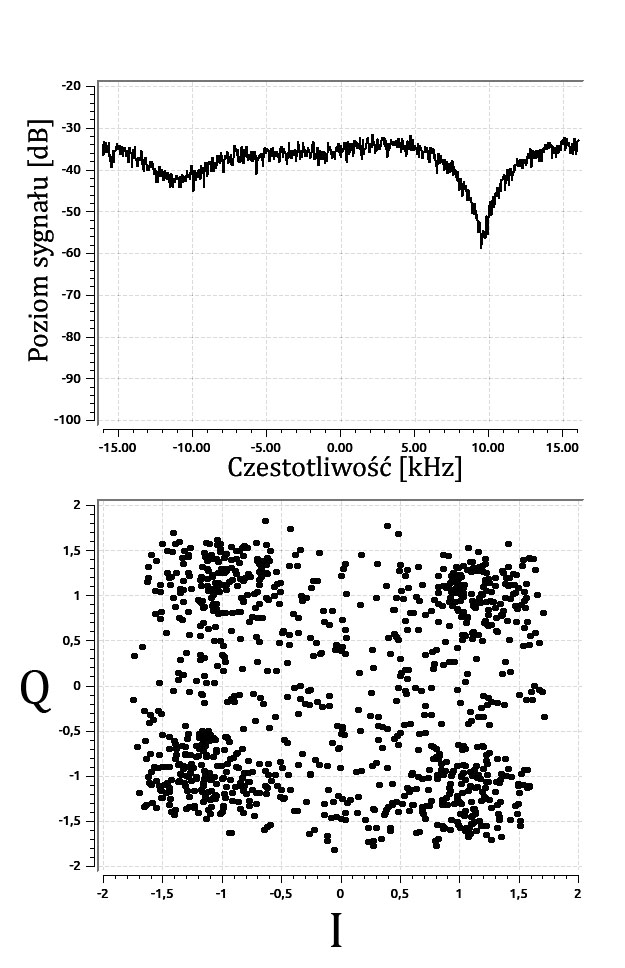
\includegraphics[scale=0.32]{channel_noeq}      & 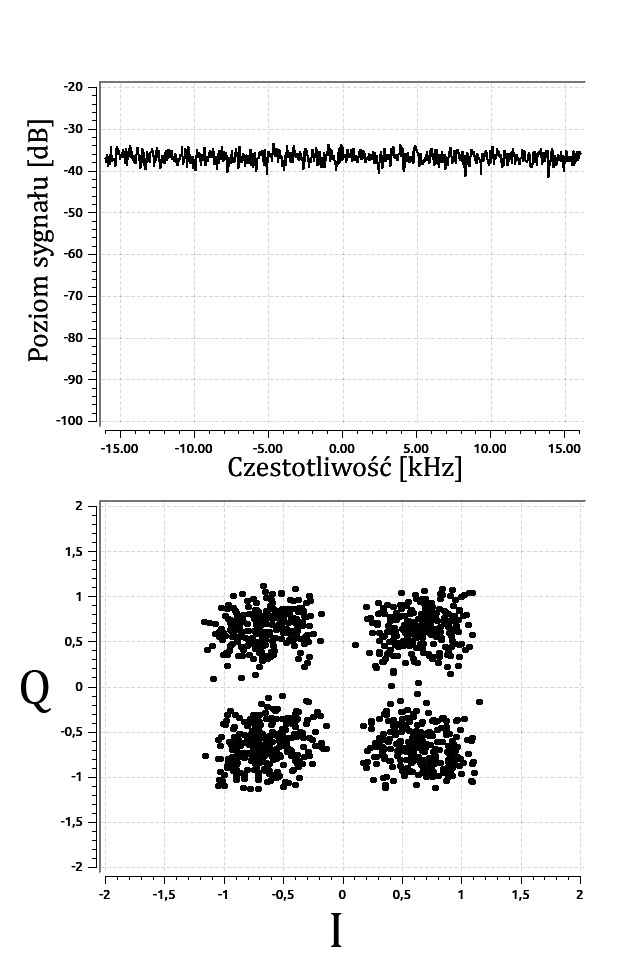
\includegraphics[scale=0.32]{channel_eq}      \\ \hline
\end{tabular}
\end{table}




